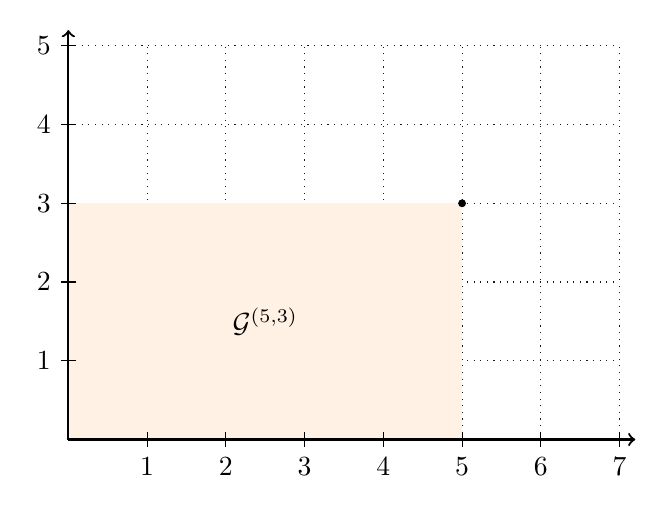
\begin{tikzpicture}
    \draw[black!90,dotted] (0,0) grid (7,5);
    \fill[orange!10] (0,0) rectangle (5,3);
    \draw[thick,->] (0,0) -- (7.2,0);
    \draw[thick,->] (0,0) -- (0,5.2);
    \foreach \x in {1,...,7} {%
        \draw (\x,.1) -- (\x,-.1) node[below] {$\x$};
    }
    \foreach \y in {1,...,5} {%
        \draw (.1,\y) -- (-.1,\y) node[left] {$\y$};
    }
    \fill (5,3) circle (0.05);
    \draw (2.5,1.5) node {$\mathcal{G}^{(5,3)}$};
\end{tikzpicture}